\section{Построение регрессионных моделей}

\subsection{Линейная модель \(y = a + bx\)}

\subsubsection{Оценивание параметров}

Оценки параметров линейной модели находятся методом наименьших квадратов (МНК). Введём обозначения:

\[
\bar{x} = \frac{1}{n}\sum_{i=1}^{n} x_i = 1128.963, \quad
\bar{y} = \frac{1}{n}\sum_{i=1}^{n} y_i = 1090.963,
\]
\[
S_{xx} = \sum_{i=1}^{n}(x_i - \bar{x})^2 = 26\,186\,057.926, \quad
S_{xy} = \sum_{i=1}^{n}(x_i - \bar{x})(y_i - \bar{y}) = 25\,869\,628.926.
\]

Тогда оценки коэффициентов:

\[
\hat{b} = \frac{S_{xy}}{S_{xx}} = \frac{25\,869\,628.926}{26\,186\,057.926} = 0.9879,
\]
\[
\hat{a} = \bar{y} - \hat{b}\bar{x} = 1090.963 - 0.9879 \cdot 1128.963 = -24.358.
\]

\subsubsection{Уравнение регрессии}

Итоговое уравнение линейной регрессии:

\[
\hat{y} = \hat{a} + \hat{b}x = -24.358 + 0.9879 \, x.
\]

\subsubsection{График модели}

На рисунке~\ref{fig:linear} представлена линейная модель на фоне исходных данных.

\begin{figure}[H]
\centering
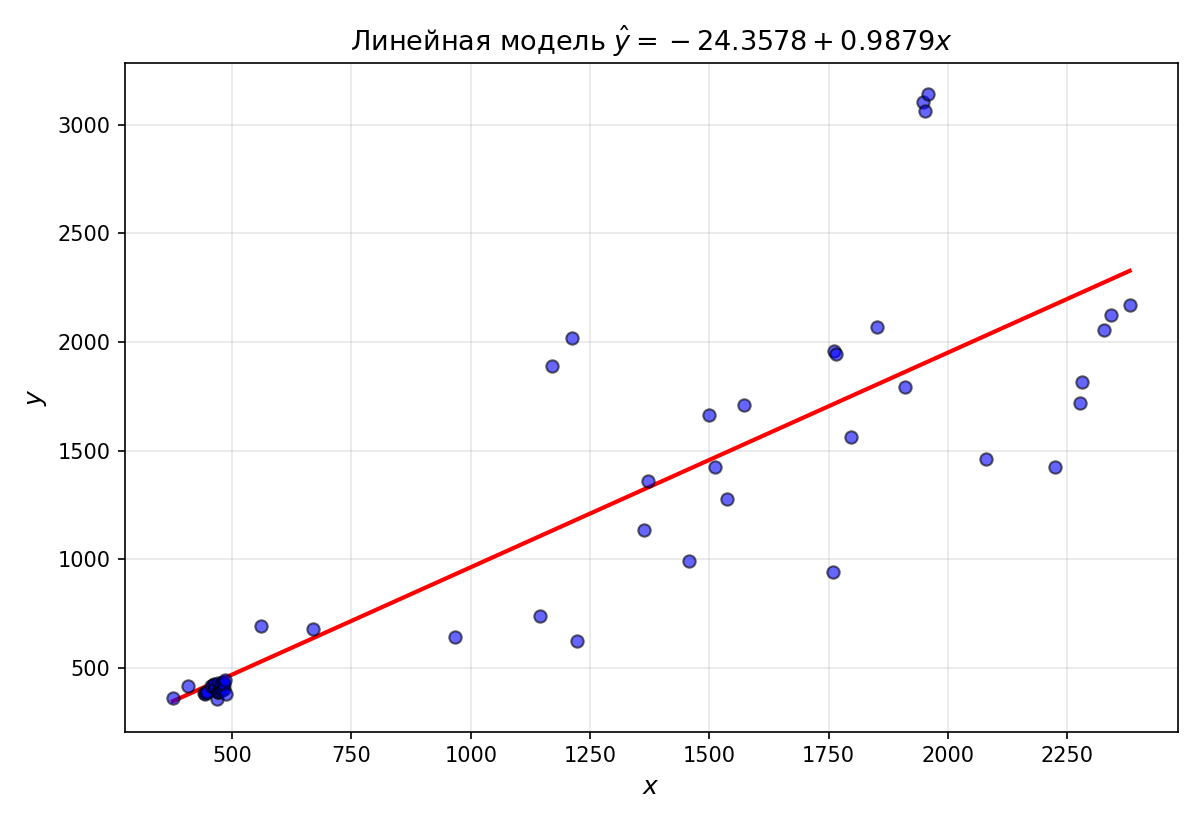
\includegraphics[width=0.65\textwidth]{linear_model.png}
\caption{Линейная модель \(\hat{y} = -24.358 + 0.9879x\)}
\label{fig:linear}
\end{figure}

\subsubsection{Интерпретация коэффициентов}

Коэффициент наклона \(\hat{b} = 0.9879\) означает, что при увеличении скорости чтения на 1 МБ/с скорость записи в среднем возрастает примерно на 0.99 МБ/с. Свободный член \(\hat{a} = -24.358\) указывает на то, что при нулевой скорости чтения прогнозируемая скорость записи формально отрицательна, однако это значение лежит за пределами диапазона наблюдаемых \(x\) (\(x \in [376, 2381]\)) и не имеет содержательной интерпретации.

\subsection{Квадратичная модель \(y = a + bx + cx^2\)}

\subsubsection{Оценивание параметров}

Для квадратичной модели используется множественная линейная регрессия с регрессорами \(x\) и \(x^2\). Оценки параметров, полученные МНК:

\[
\hat{a} = -291.300, \quad \hat{b} = 1.6032, \quad \hat{c} = -0.000243.
\]

\subsubsection{Уравнение регрессии}

Итоговое уравнение квадратичной регрессии:

\[
\hat{y} = \hat{a} + \hat{b}x + \hat{c}x^2 = -291.300 + 1.6032 \, x - 0.000243 \, x^2.
\]

\subsubsection{График модели}

На рисунке~\ref{fig:quadratic} представлена квадратичная модель на фоне исходных данных.

\begin{figure}[H]
\centering
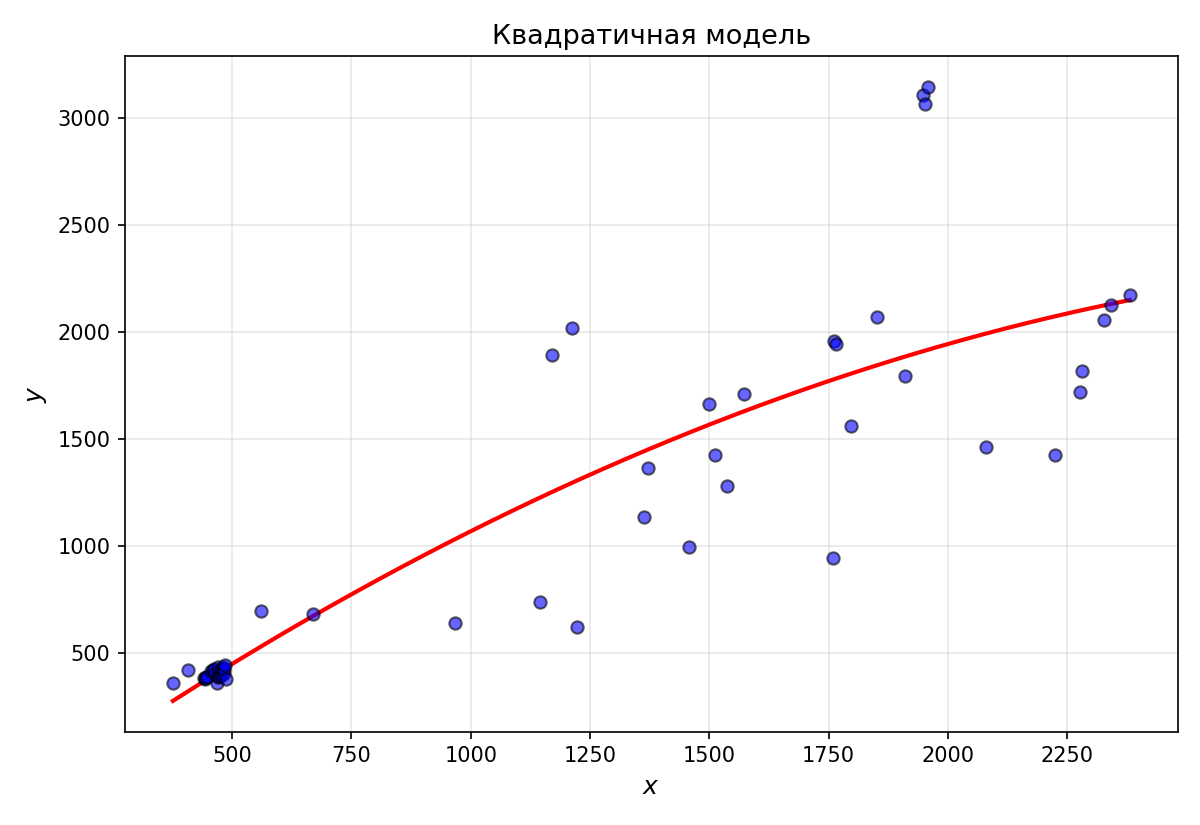
\includegraphics[width=0.65\textwidth]{quadratic_model.png}
\caption{Квадратичная модель \(\hat{y} = -291.300 + 1.6032x - 0.000243x^2\)}
\label{fig:quadratic}
\end{figure}

\subsubsection{Интерпретация}

Отрицательный коэффициент при \(x^2\) (\(\hat{c} = -0.000243\)) указывает на выпуклый вверх характер зависимости: скорость роста \(y\) с увеличением \(x\) постепенно снижается, и при достаточно больших \(x\) функция достигает максимума и начинает убывать. Однако, поскольку \(\hat{c}\) очень мал по абсолютной величине, вклад квадратичного члена становится заметным лишь при больших значениях \(x\) (порядка \(x > 1500\)).

\subsection{Степенная модель \(y = ax^b\)}

\subsubsection{Линеаризация}

Степенная модель приводится к линейному виду логарифмированием обеих частей:

\[
\ln y = \ln a + b \ln x.
\]

Введём новые переменные: \(u_i = \ln x_i\), \(v_i = \ln y_i\). Тогда модель принимает вид \(v = \ln a + b u\) — линейная зависимость \(v\) от \(u\).

\subsubsection{Оценивание параметров}

Оценки параметров находятся МНК на линеаризованных данных:

\[
\bar{u} = \frac{1}{n}\sum_{i=1}^{n} u_i = 6.8170, \quad
\bar{v} = \frac{1}{n}\sum_{i=1}^{n} v_i = 6.7266,
\]
\[
S_{uu} = \sum_{i=1}^{n}(u_i - \bar{u})^2 = 23.873, \quad
S_{uv} = \sum_{i=1}^{n}(u_i - \bar{u})(v_i - \bar{v}) = 24.834.
\]

\[
\hat{b} = \frac{S_{uv}}{S_{uu}} = \frac{24.834}{23.873} = 1.0402,
\]
\[
\widehat{\ln a} = \bar{v} - \hat{b}\bar{u} = 6.7266 - 1.0402 \cdot 6.8170 = -0.3646.
\]

Обратное преобразование даёт \(\hat{a} = e^{\widehat{\ln a}} = e^{-0.3646} = 0.6945\).

\subsubsection{Уравнение регрессии}

Итоговое уравнение степенной регрессии:

\[
\hat{y} = \hat{a} x^{\hat{b}} = 0.6945 \, x^{1.0402}.
\]

\subsubsection{График модели}

На рисунке~\ref{fig:power} представлена степенная модель на фоне исходных данных.

\begin{figure}[H]
\centering
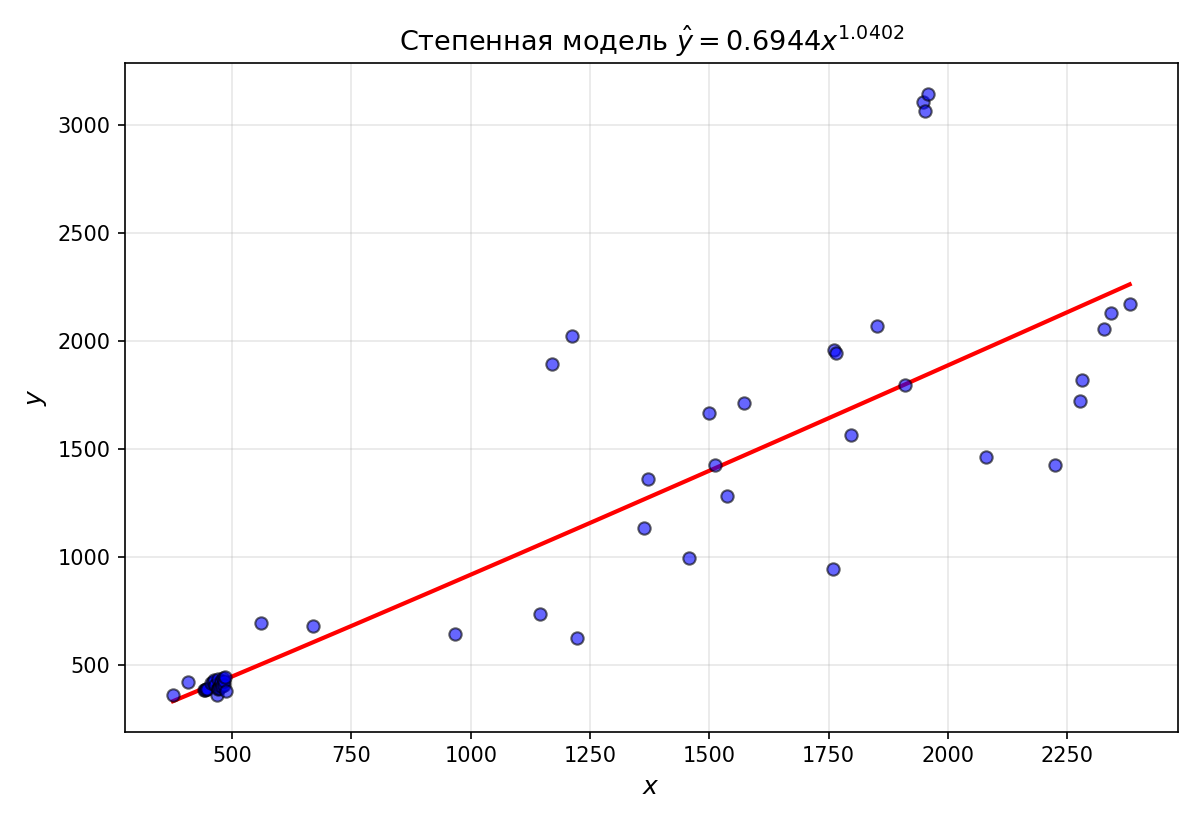
\includegraphics[width=0.65\textwidth]{power_model.png}
\caption{Степенная модель \(\hat{y} = 0.6945 \, x^{1.0402}\)}
\label{fig:power}
\end{figure}

\subsubsection{Интерпретация}

Показатель степени \(\hat{b} = 1.0402 \approx 1\) указывает на то, что зависимость скорости записи от скорости чтения близка к прямой пропорциональности. Небольшое превышение \(\hat{b}\) над единицей означает, что с ростом скорости чтения скорость записи растёт чуть быстрее линейного закона. Коэффициент \(\hat{a} = 0.6945\) является масштабным множителем.

\subsection{Прогнозные значения \(\hat{y}_i\)}

В таблице~\ref{tab:yhat_all} приведены фактические и прогнозные значения для первых десяти наблюдений по всем трём моделям.

\begin{table}[H]
\centering
\caption{Фактические и прогнозные значения (первые 10 строк)}
\label{tab:yhat_all}
\begin{tabular}{ccccc}
\toprule
\(i\) & \(y_i\) & \(\hat{y}_i^{\text{лин}}\) & \(\hat{y}_i^{\text{кв}}\) & \(\hat{y}_i^{\text{ст}}\) \\
\midrule
1 & 361.0 & 347.10 & 277.12 & 331.45 \\
2 & 419.0 & 378.71 & 322.33 & 360.85 \\
3 & 385.0 & 412.30 & 369.81 & 392.18 \\
4 & 381.0 & 413.29 & 371.20 & 393.10 \\
5 & 389.0 & 415.26 & 373.97 & 394.95 \\
6 & 390.0 & 418.23 & 378.13 & 397.72 \\
7 & 418.0 & 426.13 & 389.20 & 405.11 \\
8 & 420.0 & 429.10 & 393.34 & 407.88 \\
9 & 428.0 & 433.05 & 398.86 & 411.58 \\
10 & 407.0 & 435.02 & 401.61 & 413.43 \\
\bottomrule
\end{tabular}
\end{table}

Полные векторы \(\hat{y}_i\) для всех моделей (\(n = 54\)) вычислены и использованы при расчёте показателей качества в разделе~3.
